\chapter{Development}\label{ch:development}
This chapter describes the setup and the methods used for recording samples that have been later used
in testing the filtering method.
\section{Microphones}
Out of all the possible choices, omnidirectional microphones were used. Some advantages of this 
type of microphones are represented by the face that they have a flat frequency response, meaning 
they deliver the same electrical output no matter what the angle of incidence. This was crucial to us
since different angles were used in recording the samples.\cite{MICROPHONE}

\begin{figure}[htp]
	\centering
	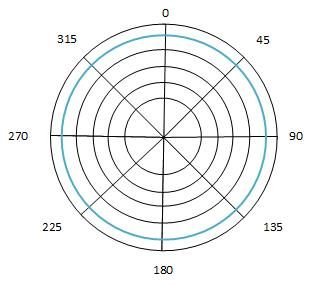
\includegraphics[width=0.5\textwidth]{Illustrations/omnidirectional.jpg}
	\caption{Omnidirectional Microphone Electrical Output}
	\label{fig:omniMic}
\end{figure}
Figure \ref{fig:omniMic} represents the electrical output of the microphone, in relation to the angle of
incidence.
\newpage
\section{Distancing}
In order to detect a delay between the sound signals, a certain distance between the microphones was
necessary. Different distances between the microphones were used in different recording sessions.
This poses advantages and disadvantages.
For once, a higher distance between the microphones,
would result in higher delay, thus giving a better accuracy. However, by increasing the distance,
the gain of one of the signals reaching one microphone, would significantly increase over the other. 
This poses a problem when trying to separate the signals.
\section{Environment}
As an anechoic room was unavailable, the recordings were taken in one of the rooms available at the university. 
The sound sources around the room were dampened as much as possible, in an attempt to get clear and accurate 
recordings.
\section{Sampling} 
A high enough sampling frequency was needed, due to two reasons. Firstly, a higher sampling frequency
gives a higher accuracy in delay samples. Secondly, in order to avoid aliasing. 48kHz was used
as sampling frequency. This gives the highest accuracy that the microphones can provied, and is also
high enough to avoid aliasing.\cite{SAMPLINGFREQUENCY}
\newpage
\section{Setup}
Figure \ref{fig:RanzvanRecSetup} represents the setup used. The microphones have been put up at a
approximate height as the speakers mouth, in order to more accurately capture the delay.

\begin{figure}[htp]
	\centering
	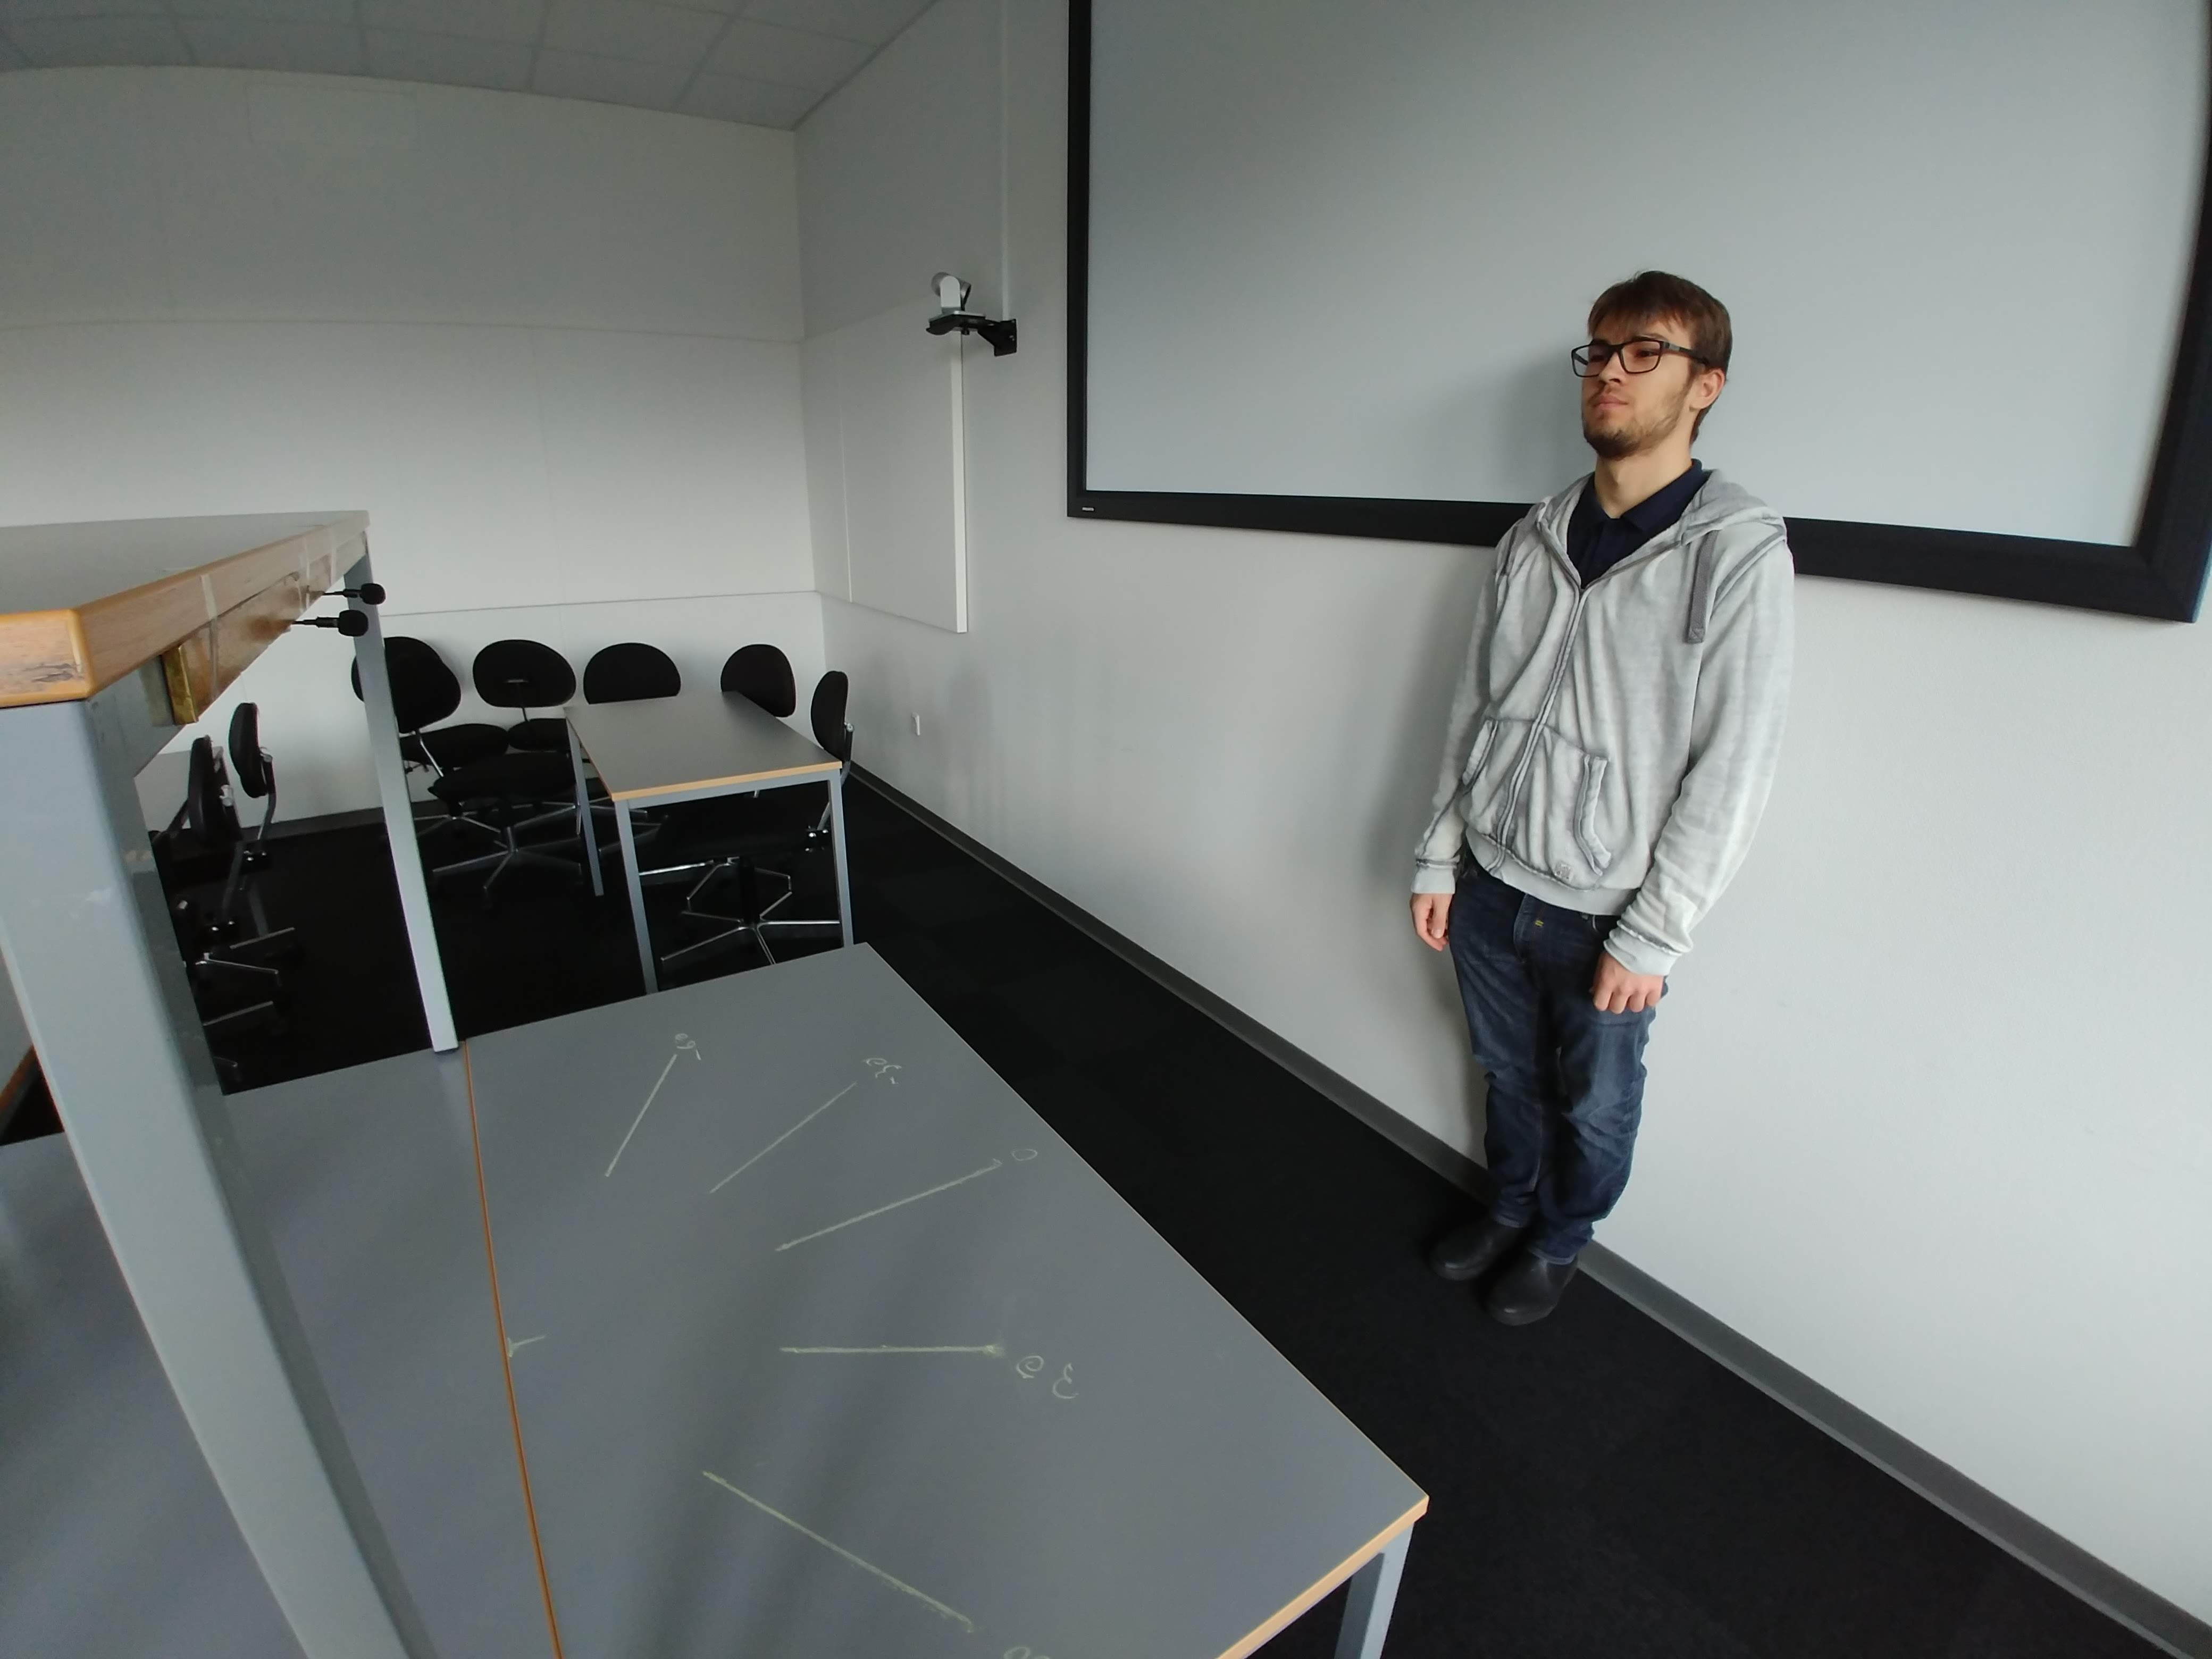
\includegraphics[width=\textwidth]{Illustrations/razvanWithSetup.jpg}
	\caption{Microphone Setup}
	\label{fig:RanzvanRecSetup}
\end{figure}

Although this height might vary in real life scenarios, the same height was used throughout multiple recording
sessions due to simplicity.

Different recording scenarios were considered, involving one, two or three persons, acting as sound sources,
coming from different angles.

Filtering was attempted on all of them, with different results obtained.
\newpage
Figure \ref{fig:recSetup} shows the approximate angles at which different recording were taken. Knowing the 
angles was important for us to be able to test the filtering method.

\begin{figure}[htp]
	\centering
	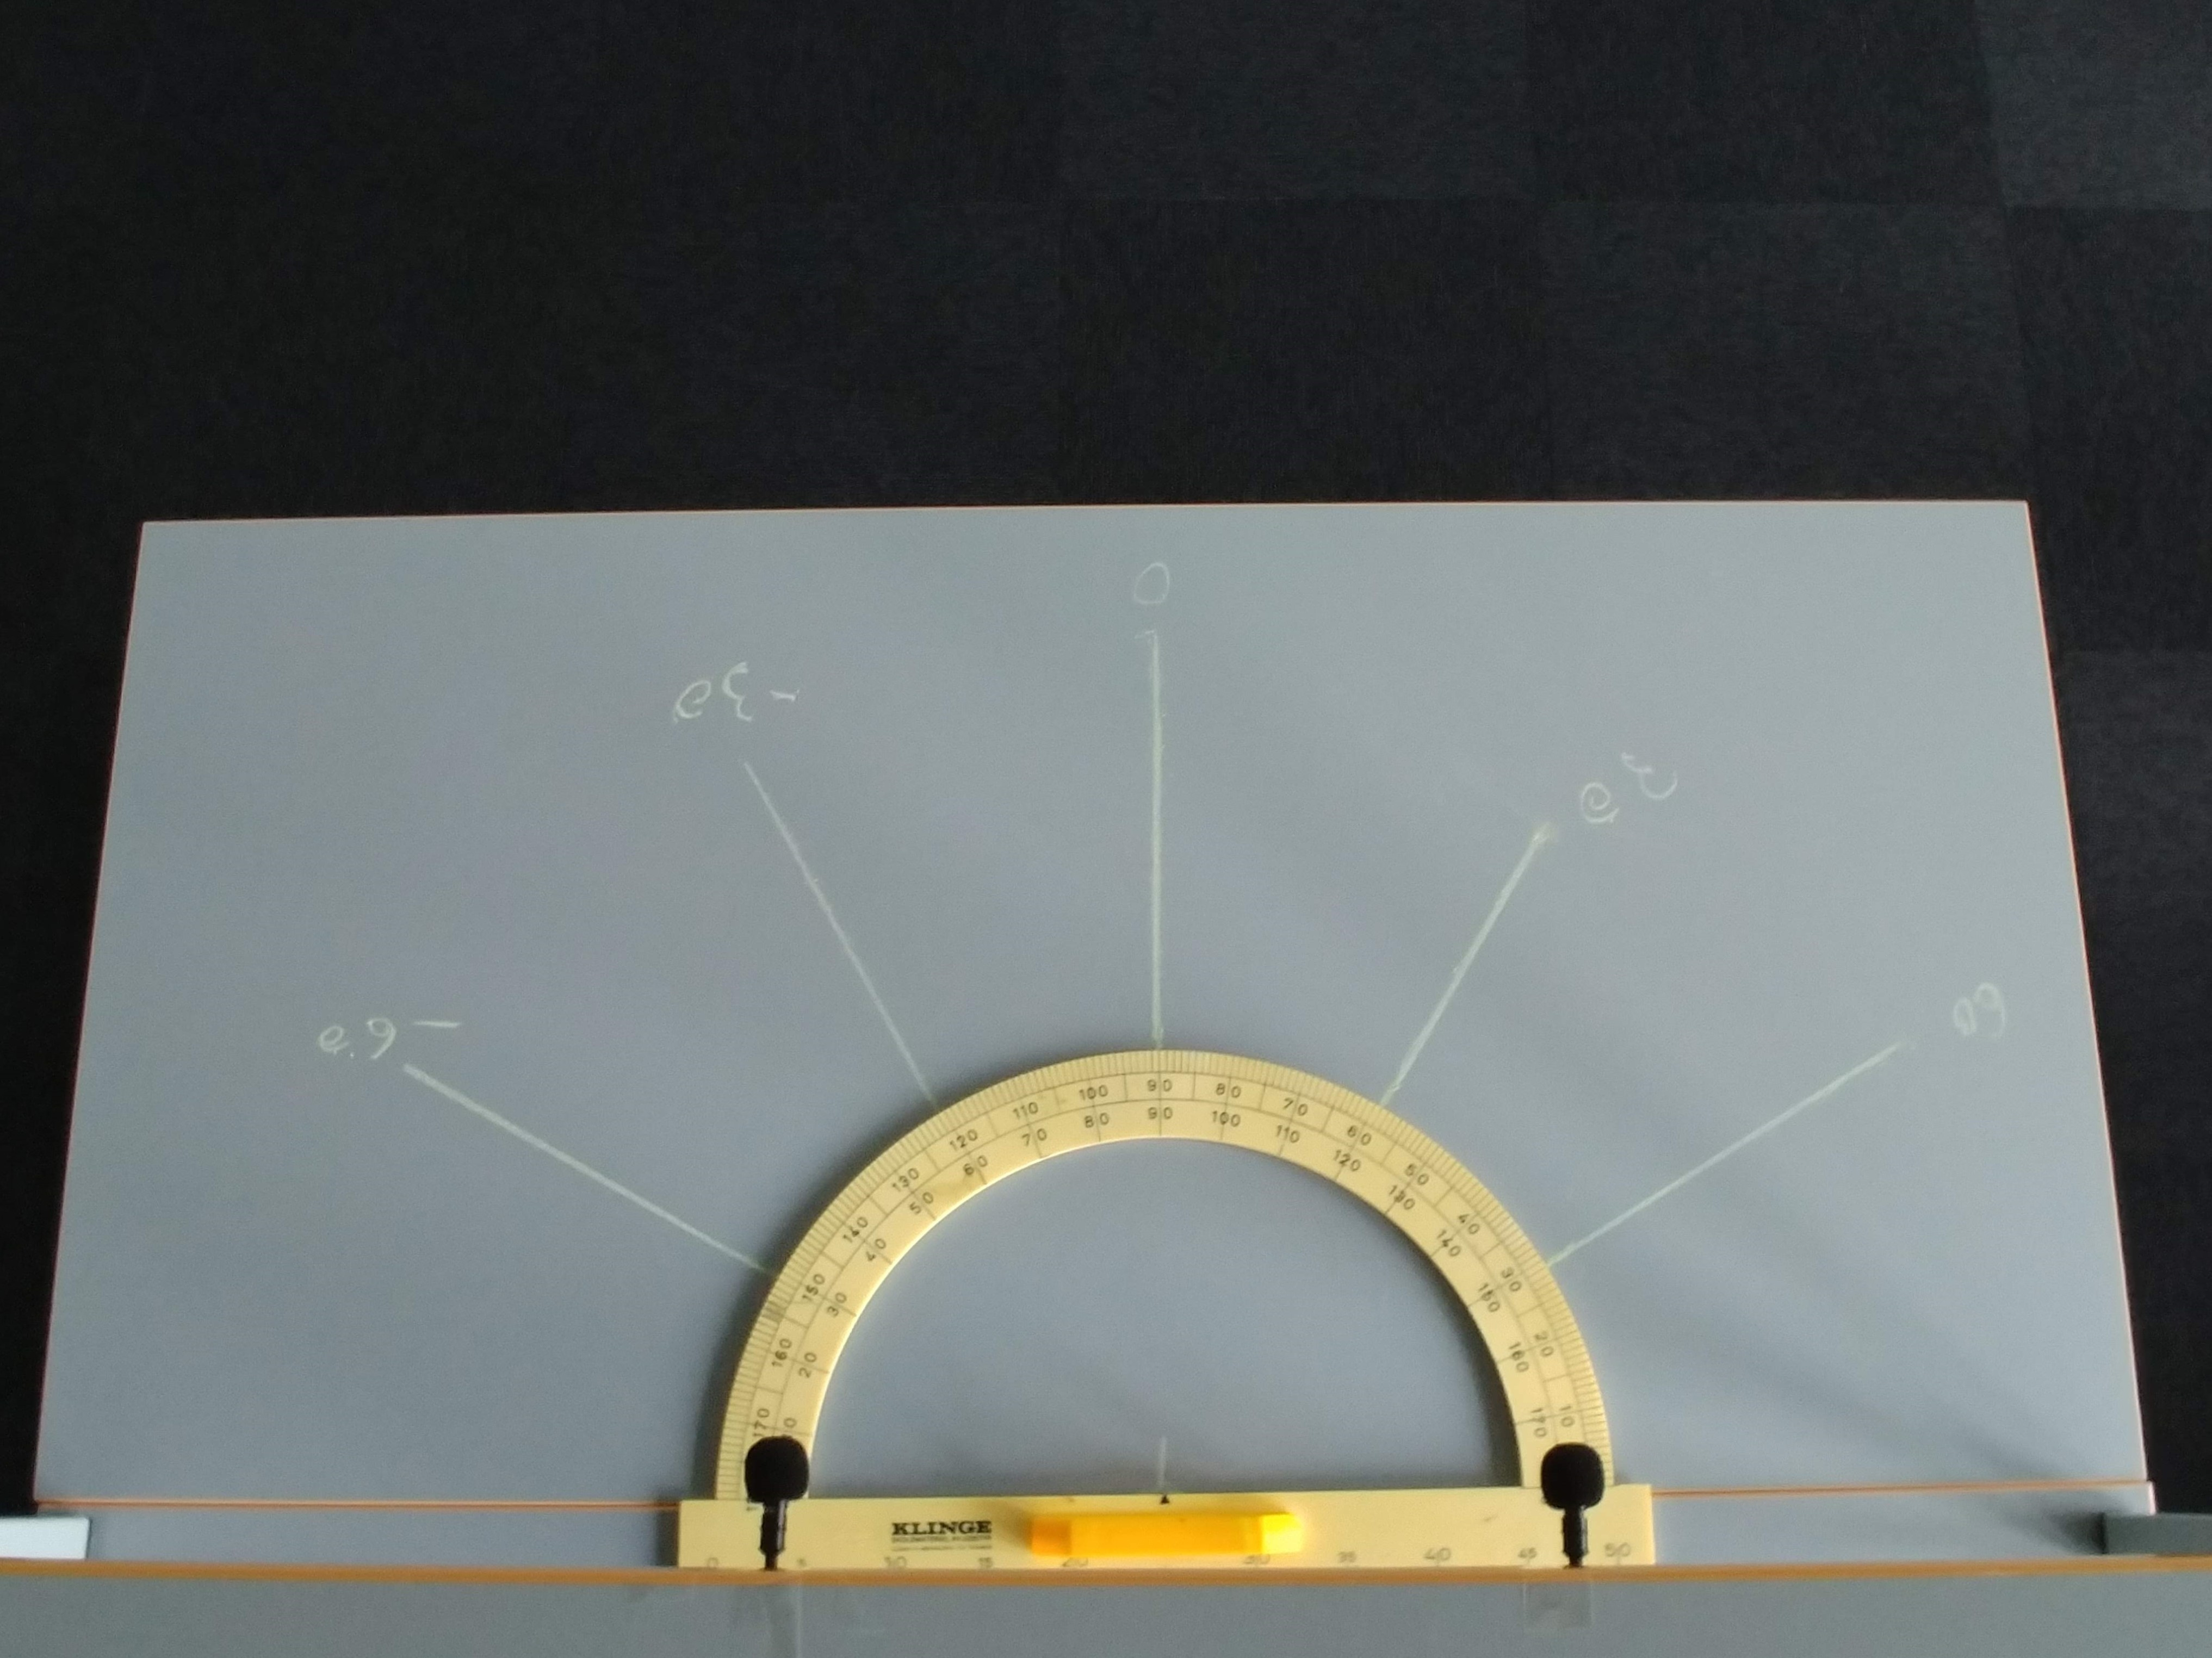
\includegraphics[width=1\textwidth]{Illustrations/JustSetup.jpg}
	\caption{Setup for Recording}
	\label{fig:recSetup}
\end{figure}